\documentclass{beamer}
%\usetheme{Madrid} % My favorite!
\usetheme{Boadilla} % Pretty neat, soft color.
%\usetheme{default}
%\usetheme{Warsaw}
%\usetheme{Bergen} % This template has nagivation on the left
%\usetheme{Frankfurt} % Similar to the default with an extra region at the top.
\usecolortheme{seahorse} % Simple and clean template
%\usetheme{Darmstadt} % not so good
% Uncomment the following line if you want %
% page numbers and using Warsaw theme%
% \setbeamertemplate{footline}[page number]
%\setbeamercovered{transparent}
\setbeamercovered{invisible}
% To remove the navigation symbols from 
% the bottom of slides%
\setbeamertemplate{navigation symbols}{} 
%
\usepackage{graphicx}
%\usepackage{bm}         % For typesetting bold math (not \mathbold)
%\logo{\includegraphics[height=0.6cm]{curve.eps}}
%
\title[EVE: Efficient Vector Encryption]{EVE: An Implementation of an Efficient \\ Homomorphic Encryption Scheme on Integer Vectors}
\author[Yu, Lai, Payor]{Angel Yu \\ Wai Lok Lai \\ James Payor}
\institute[MIT]
{
%18.100C \LaTeX \,Exercise 2 \\
%\medskip
%{\emph{}}
}
\date{\today}
\usepackage{mathrsfs}
\usepackage{setspace}
\usepackage{amsmath, amssymb, amsthm, enumerate}
\usepackage{lmodern} %sf font

\newcommand{\fm}[1]{\begin{align*}#1\end{align*}} %general
\newcommand{\enumn}[1]{\begin{enumerate}[(1)]#1\end{enumerate}} %general
\newcommand{\enuma}[1]{\begin{enumerate}[(a)]#1\end{enumerate}} %general
\newcommand{\enumi}[1]{\begin{enumerate}[(i)]#1\end{enumerate}} %general
\newcommand{\itz}[1]{\begin{itemize}#1\end{itemize}} %general
\newcommand{\cas}[1]{\begin{cases}#1\end{cases}} %general
\newcommand{\bs}{$\blacksquare$} %general
\newcommand{\ws}{$\qed$} %general
\newcommand{\es}{\exists} %general
\newcommand{\ve}{\varepsilon} %general
\newcommand{\vp}{\varphi} %general

\newcommand{\ii}[1]{\emph{\textsf{#1}}} %6437
\newcommand{\iik}{\emph{\textsf{k}}} %6437
\newcommand{\iis}{\emph{\textsf{s}}} %6437
\newcommand{\iiw}{\emph{\textsf{w}}} %6437
\newcommand{\iix}{\emph{\textsf{x}}} %6437
\newcommand{\iiy}{\emph{\textsf{y}}} %6437
\newcommand{\iiz}{\emph{\textsf{z}}} %6437
\newcommand{\iih}{\emph{\textsf{H}}} %6437
\newcommand{\bbc}{{\bf c}} %6437
\newcommand{\bbe}{{\bf e}} %6437
\newcommand{\bbx}{{\bf x}} %6437
\newcommand{\vb}{\textbar} %6437
\newcommand{\gel}{\gtreqless} %6437
\newcommand{\gl}{\gtrless} %6437






\begin{document}



\begin{frame}
\titlepage
\end{frame}






\begin{frame}
\frametitle{Introduction to Homomorphic Encryption}

\begin{figure}[ht]
\centering
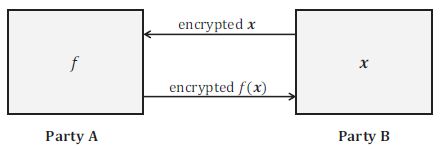
\includegraphics[width=3.2in]{he}
\caption{Most common usage of homomorphic encryption schemes}
\end{figure}

\begin{figure}[ht]
\centering
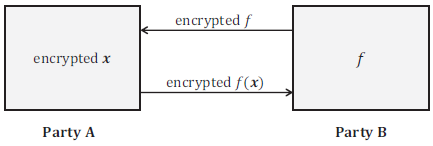
\includegraphics[width=3.2in]{eve}
\caption{EVE, the homomorphic encryption scheme considered in our project}
\end{figure}
\end{frame}





\begin{frame}{Overview of EVE: Supported Operations}
Fundamental Operations: 
\itz{
\item{Encrypt: $\bbc = E_S(\bbx)$}
\item{Decrypt: $\bbx = D_S(\bbc)$}
\item{Switching secret keys from $S$ to $S'$}
}
\vspace{.15in}
Supported Operations on Integer Vectors: 
\itz{
\item{Addition of two vectors: $\bbx_1 + \bbx_2$}
\item{Linear transformation: $G\bbx$}
\item{Weighted inner product of two vectors: $\bbx_1^T H \bbx_2$}
}
\vspace{.15in}
Can compose these operations to support arbitrary integer polynomials
\end{frame}




\begin{frame}{Details of Fundamental Operations}
Encrypt $\bbx$ with secret key $S$:
\itz{
\item{ Choose $\bbc$ such that $S\bbc = w\bbx + \bbe$ }
}
\vspace{.15in}
Decrypt $\bbc$ with $S$:
\itz{
\item{$\bbx = \left\lceil \frac{S\bbc}{w} \right\rfloor$}
}
\vspace{.15in}
Key switching from $S$ to $S'=[I,T]$:
\itz{
\item{Want $S'\bbc' = S\bbc$}
\item{Want key-switch matrix $M$ such that $S'M=S+E$}
\item{$M=\begin{pmatrix}
-TA + S + E \\
A 
\end{pmatrix}$ for random matrix $A$, random noise matrix $E$}
\item{Then $\bbc'=M\bbc$}
}
\end{frame}





\begin{frame}{Details of the Three Supported Operations}
Addition: $\bbx' = \bbx_1 + \bbx_2$:
\itz{
\item{Let $\bbc' = \bbc_1 + \bbc_2$}
\item{So $S\bbc'=w(\bbx_1+\bbx_2)+(\bbe_1+\bbe_2)$}
}
\vspace{.15in}
Linear Transformation: $\bbx' = G\bbx$
\itz{
\item{Note $GS\bbc = wG\bbx + G\bbe$}
\item{Hence $E_S(\bbx) = E_{GS}(G\bbx)$}
\item{So $\bbc'=\bbc$ and decrypt with $S' = GS$}
}
\end{frame}




\begin{frame}{Details of the Three Supported Operations (con'd)}
Weighted Inner Product: $\bbx' = \bbx_1^T H \bbx_2$
\itz{
\item{Let $S'=\text{vec}(S^T H S)^T $}
\item{Let $\bbc'=\left\lceil \frac{\text{vec}(\bbc_1 \bbc_2^T}{w} \right\rfloor$}
\vspace{.07in}
\item{Note $(S\bbc_1)^T H (S\bbc_2) = w^2(\bbx_1^T H \bbx_2)+(w\bbx_1^T H \bbe_2 + w\bbe_1^T H \bbx_2 + \bbe_1^T H \bbe_2)$}
\vspace{.07in}
\item{So $S'\bbc' = w(\bbx_1^T H \bbx_2) + \bbe'$}
}
\end{frame}





\begin{frame}
\frametitle{Secrecy in the Scheme}

\itz{
\item{ Clients (Party B) calculate key-switch matrices based on operation $f$}
\item{ Server (Party A) performs the operation without knowing $f$}
\item{ Relies on key-switch matrices being indistinguishable from random}

}
	
\begin{block}{Learning with Error Problem (LWE)}
\begin{center}
Given $S$ and $M$, solving $S'M = S + E$ to find $S'$ is hard
\end{center}
\end{block}

\vspace{.07in}
\begin{figure}[ht]
\centering
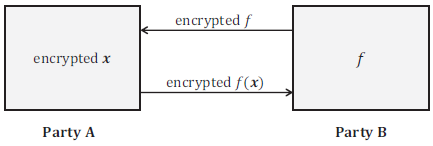
\includegraphics[width=3.2in]{eve}
\end{figure}
\end{frame}



\begin{frame}
\frametitle{Applications}

\itz{
\item{In each application, we have:
 \itz{
 	\item{Server with data (can be encrypted with $S$, known to the client)}
 	\item{Client that wants to learn a function of the data}
 	}
 }
\vspace{.15in}
\item{Effective when server has a lot of data, and results are small}
}
\end{frame}





\begin{frame}
\frametitle{Applications}

\itz{
\item{Search
 \itz{
 	\item{Server has (encrypted) feature vectors for our data}
 	\item{Client wants to score each item to rank them}
	}
 }
\vspace{.1in}
\item{Classification
	\itz {
		\item{Can run any polynomial classifier on the server's data (e.g. naive bayes, SVMs with polynomial kernels)}
	}
}
\vspace{.1in}
\item{Feature extraction
	\itz {
		\item{We can generalize classification to give a low-dimensional representation of data vectors, which will conserve bandwidth over simply querying all the files.}
	}
}
}
\end{frame}







\begin{frame}
\frametitle{Demo}
\itz{
\item{We implemented the scheme, and two applications:}
\vspace{.05in}
\itz{
	\item{Private search on encrypted data \\(using TF-IDF relevance on common words)}
	
\vspace{.05in}
	\item{Spam classification (using a naive-bayes model)}
}
\vspace{.1in}
\item{Server has encrypted word counts of 3500 common words for 200 Enron emails}
\vspace{.1in}
\item{Server can't learn our queries, or even distinguish between each type}
}
\end{frame}


\begin{frame}
\frametitle{Live Demo!}
\begin{figure}[ht]
\centering

\includegraphics[width=3.5in]{live}
\end{figure}
\end{frame}


\begin{frame}
\frametitle{Conclusions}
\itz{
\item{In our demo, scheme is slow due mainly to our lack of optimization.}
\vspace{.1in}
\item{No overhead in addition}
\item{Multiplicative overhead in linear transformations and inner products equal to the number of bits involved.
	\itz{
		\item{(Note as given, inner products is slow, but we can combine this with a linear transformation step to reduce the work.)}
	}
}
\vspace{.1in}
\item{This scheme compares well to fully homomorphic encryption by limiting scope of computation.
	\itz{
		\item{Benchmarks give that HElib achieves ~500 multiplications per second for small integers, orders of magnitude worse than our slowdown.}
	}
}
}
\end{frame}


\begin{frame}
\frametitle{Questions?}
\begin{figure}[ht]
\centering

\includegraphics[width=3.5in]{questions}
\end{figure}
\end{frame}




\end{document}